% master file siminos/froehlich/slice/chart.tex
% $Author$ $Date$

% \section{Charting the \reducedsp}
%       \label{sec:chart}


So far, the good news is that for a generic {\template} $\slicep$ (\ie,
any $\slicep$ whose group orbit has the full $N$-dimensions of the group
\Group), the slice hyperplane \refeq{PCsectQ} cuts across the group orbit
of {\em every} point in the full \statesp\ \pS. But is this a useful
symmetry reduction of the full \statesp? A distant pattern that is a bad match
to a given {\template} will have any number of locally `minimal'
distances, each yet another bad match.
Even though every generic slice cuts all group orbits, it makes no sense
physically to use one slice (a set of all group orbit points that are
closest to one given {\template}) globally.
A slice
defined here is a purely group-theoretic, linear construct, with no
reference to dynamics; a given {\template} \slicep\ defines the
associated slice, a ($d\!-\!N$)\dmn\ hyperplane. Within it, there is a
($d\!-\!N\!-1$)\dmn\ singularity hyperplane
\[
\braket{\groupTan(\sspSing)}{\sliceTan{}}=0
\]
where the group tangent of a point $\sspSing=\LieEl^{-1} \ssp$ lies in
the slice. If we pick another slice-fixing point $\slicep'$, it comes
along with its own slice and singularity hyperplane.
Work on \KS\ suggests how to
proceed: the main advance of \refref{lanCvit07} was to show that for more
turbulent/chaotic systems a set of Poincar\'e sections is needed to
capture the dynamics. Sets of {\PoincSec}s are picked so each captures a
neighborhoods of an important, qualitatively distinct class of solutions
(2-rolls states, 3-rolls states). The choice should be `physical,'
dictated by the dominant patterns seen in the solutions of nonlinear
PDEs.
	\PC{
	Awkward: cannot use most \eqva\ as `templates,' as they often
	are invariants under subgroups of the symmetry group \Group, and
	thus their group orbits have dimensions less than $N$.
	}

So idea is to
coarsely cover the nonlinear strange attractor with a set of hyperplanes,
as in \reffig{fig:Tesselate}. For any pair, they intersect in a
`ridge,' a
boundary hyperplane of one less dimension. So our task is to, for a
given strange attractor, pick a set of slice-fixing points, such that
each is approximately tangent to the strange attractor, and the
singularity hyperplanes are eliminated by requiring that they lie either
on the `wrong' side of the slice-slice intersection, or somewhere where
the strange attractor does not tread.

Our proposal is to approximately
% \HREF{http://en.wikipedia.org/wiki/Voronoi_tessellation}
{Voronoi
tessellate}  the curved manifold in which the reduced strange attractor
is embedded by a finite set of hyperplanes\rf{RoSa00}, each a slice
tangential to one of a finite number of `reference states' or
{\template}. This tessellation is akin to the
%\HREF{http://en.wikipedia.org/wiki/Vector_quantization}
{`vector quantization,'} (`block quantization,'  `pattern matching quantization'),
a computer science data compression method where sets of points are
clustered by their distance to `prototype' or `reference' points. The
method encodes values from a multidimensional vector space into a
`codebook,' a finite set of values from a discrete space of a lower
dimension; \ie, what in the theory of dynamical systems is called
`symbolic dynamics.'

So how do we propose to implement this tessellation?

% in part clipped from
% www.cs.unm.edu/~terran/downloads/classes/cs529-s10/docs/pretest_soln.pdf
An (affine) hyperplane is the locus of points obeying the equation:
\[
\sspRed_1\sliceTan{1} + \sspRed_2\sliceTan{2} + \cdots + \sspRed_d\sliceTan{d} = c
\,.
\]
\ie, $\braket{\sspRed}{\sliceTan{}}=c$. In the case of a slice, the
extremal distance condition \refeq{PCsectQ0} sets $c=0$, so all our
slices include the point at the origin, $\sspRed=0$. A $(d\!-\!1)$\dmn\
hyperplane $\pSRed{}^{(j)}$ embedded in a $d$\dmn\ space and passing
through the origin is defined by the normal vector $\sliceTan{}{}^{(j)}$,
a vector orthogonal to every vector in the hyperplane (the tangent space
\sliceTan{} is the primary object, the {\template} \slicep\ secondary in
this way of thinking). The intersection of two $(d\!-\!1)$\dmn\
hyperplanes is a $(d\!-\!2)$\dmn\ hyperplane - the `ridge' (`boundary,'
`edge'), a hyperplane which also goes through the origin. If an ant is
crawling along the trajectory $\sspRed{}^{(1)}(\tau)$ symmetry-reduced
with respect to the first slice $\pSRed{}^{(1)}$, you do not need to
compute the precise location of this ridge. The moment
$\braket{\sspRed{}^{(1)}(\tau)}{\sliceTan{}{}^{(2)}}$ changes sign, the
ant has crossed the ridge, we symmetry-reduce with respect to the second
slice, and the ant continues its merry stroll along the second slice
$\pSRed{}^{(2)}$. We do not need to be very precise about the instant
where we switch, as long as we are away from either slice's singularity
subspace.

There is a rub, though - you have to figure out how to pick the phases of
different {\template s} in such way that you
minimize the distance from one to the next as you cross the ridge.
The {\em relative phases} of different \reqva\ are fixed, and, as
proposed in \refref{SCD07}, the shortest heteroclinic connections
can provide the bridge from one neighborhood to the next.

We need to make a global chart by deploying both linear slices and linear
Poincar\'e sections in neighborhoods of the most important (relative)
equilibria and/or (relative) periodic orbits (those are tricky, because
slice fixing points must lie in the full \statesp, and have no symmetry,
so most of the solutions we have are not good as they stand). This is the
periodic-orbit generalization of the idea of
{\statesp\ tessellation}
so dear to a professional cyclist, \reffig{fig:Tesselate}.

% In FrCv11.tex replaced by f_1_08_1.png
%{Hyp} %{fig6} and {tr:fig6} in ChaosBook
% \HREF{http://chaosbook.org/overheads/trace/Tesselate.jpg}
%%%%%%%%%%%%%%%%%%%%%%%%%%%%%%%%%%%%%%%%%%%%%%%%%%
 \begin{figure}
 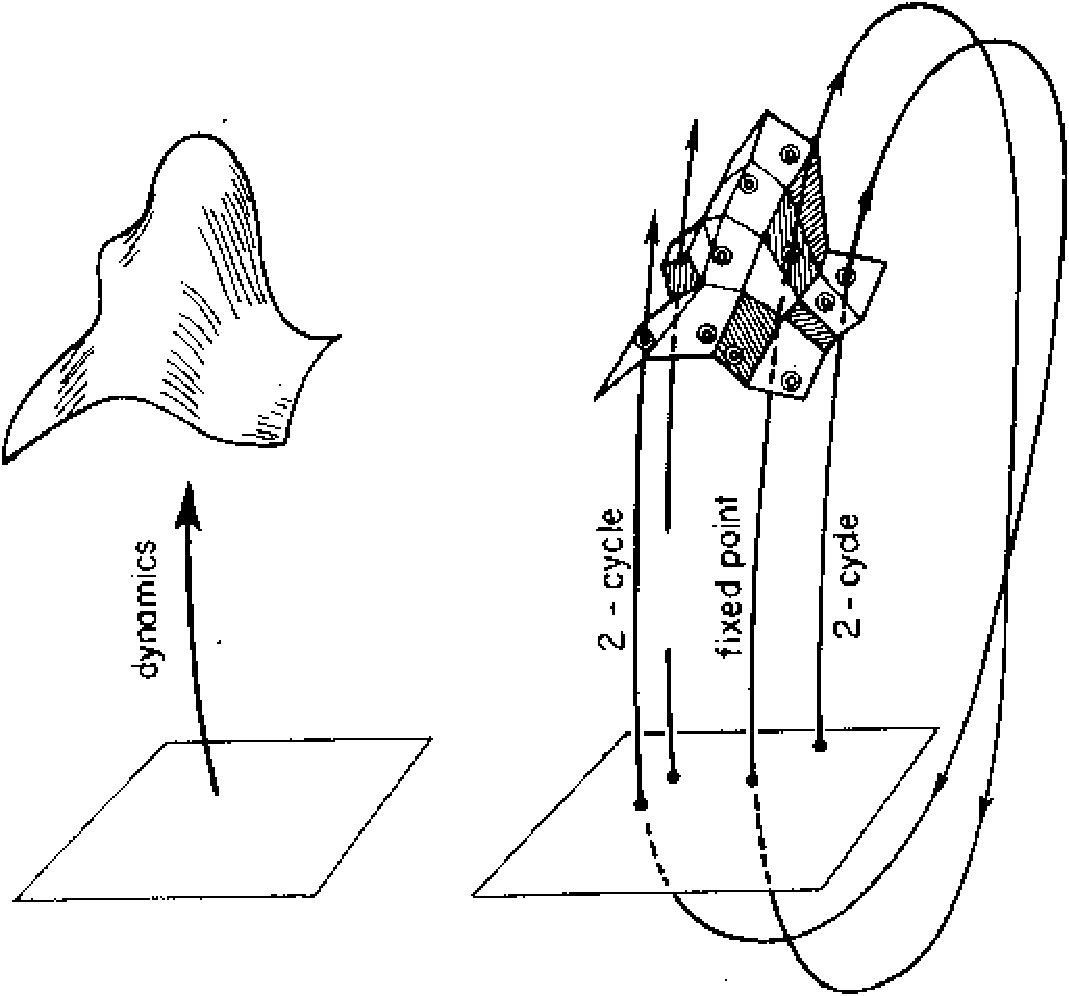
\includegraphics[width=0.35\textwidth]{f_1_08_1}
 \caption{\label{fig:Tesselate}
Smooth dynamics  (left frame) tesselated by the skeleton of
periodic points, together with their linearized neighborhoods,
(right frame).
Indicated are segments of two 1-cycles and a 2-cycle that
alternates between the neighborhoods of the two 1-cycles,
shadowing first one of the two 1-cycles, and then the other.
(From \wwwcb{}.)
  }\end{figure}
%%%%%%%%%%%%%%%%%%%%%%%%%%%%%%%%%%%%%%%%%%%%%%%%%%
%


The ridges (boundaries
between hyperplanes) are themselves hyperplanes of one dimension less,
easy compute once we have decided on the set of slices. To find
what slice a given full \statesp\ trajectory point is in, one group-rotates
with respect to each slice, and checks whether the given group orbit
belong to it. In the \reducedsp\ the trajectory is integrated within a
given slice until it hits a ridge - then one switches to
the next slice across the ridge. This passage does not need to
be computed very precisely, as long as the singularity
hyperplanes are kept a safe distance away. Ridges are of Lebesgue
measure zero, no
way you would hit them.

Global chart should be sufficiently fine-grained that we never hit any
slice singularities. That means that the neighborhood - bounded by
intersections with neighboring slices is sufficiently small that group
tangent space is nowhere within the part of the slice explored by
the strange attractor - works for smooth flows
with sufficiently small neighborhoods.

It should be emphasized that the proposed atlas retains the full
dimensionality of \reducedsp; the full dynamics is faithfully retained,
we are \emph{not} constructing a lower-dimensional model of the dynamics.
Neighborhoods of unstable \eqva and \po s are dominated by their unstable
and least contracting stable eigenvalues and are -for all practical
purposes- low-dimensional. Traversal of the ridges is, however, higher
dimensional - one is crossing from a neighborhood of, let's say, two
rolls into a neighborhood of, let's say, three rolls, and that involves
going through a pattern `defect' or a rapid transient. Nevertheless, the
recent progress on separation of `physical' and `hyperbolically isolated'
covariant Lyapunov
vectors\rf{PoGiYaMa06,ginelli-2007-99,YaTaGiChRa08,TaGiCh09} gives us
hope that proposed atlas could provide a systematic and controllable
frame lower-dimensional model of the dynamics.

%
% ****** End of file chart.tex ******
